\documentclass[11pt]{article}
\usepackage{pdfpages}
\usepackage{times}
\usepackage[margin = 0.5in]{geometry}
\usepackage[utf8]{inputenc}

\begin{document}
% frontmatter
\title{A proposal towards proposed research in computational biology}
\date{06 November 2017}
\author{Graham Voysey (gvoysey@bu.edu)\\
	    Kat Elkind (kelkind@bu.edu)\\
	    Rachel Petherbridge (rpether@bu.edu)\\
	    Kestutis Subacius (kestas@bu.edu)}
\maketitle
% main text
\section{Specific Aims}
% 1 paragraph summary of the background of the project, the key problem or question, and a statement of the overall goals of the project.
% 2-3 paragraphs describing each specific aim of the project.  Aims should be highly focused.
\section{Project Description}

	\subsection{Significance}
% why is the proposal important? how will it advance the field? what is the key problem we adddress? why do we care? 1 page or less.
	\subsection{Innovation}
% how is our approach new and unique? how does this project use and extend computational methods in a novel way
	\subsection{Research Strategy}
% what we do and how. background, approach for each aim in turn.  provide enough detail to evaluate liklihood of success.  think through potential problems and address them. include sections on dataset availabliltiy, special resources to be used, and a timeline.  Include a collaboration plan, roles of individual investigators, and specific coordination of activities to ensure group success.
		\subsubsection{Background}

		\subsubsection{Aim 1...n}

		\subsubsection{Resources}

		\subsubsection{Timeline}

		\subsubsection{Collaboration Plan}
		Work will be organized using Github (SF, CA) and the 
\newpage
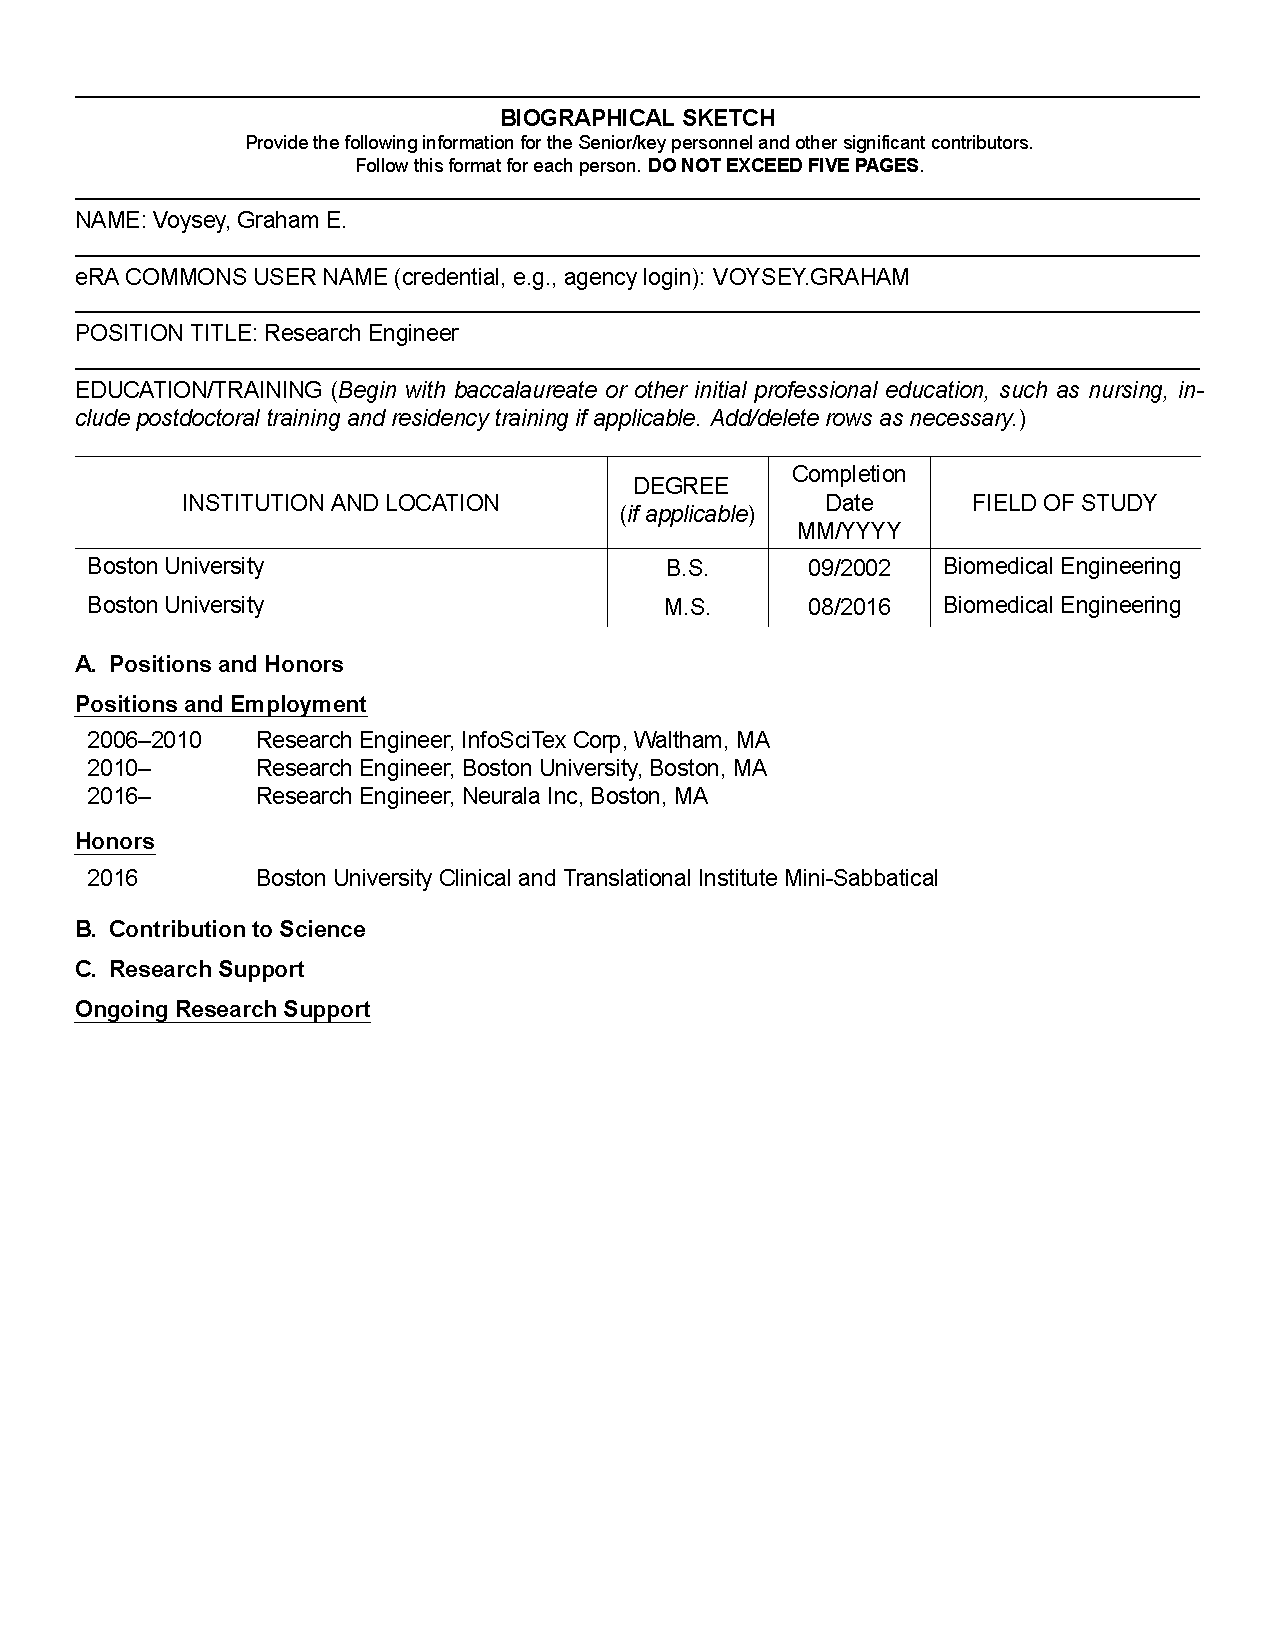
\includepdf{biosketches/gvoysey-biosketch.pdf}
% \includepdf{biosketches/kelkind-biosketch.pdf}
% \includepdf{biosketches/rpether-biosketch.pdf}
% \includepdf{biosketches/kestas-biosketch.pdf}

\end{document}